\subsubsection{Visualizzazione documento}
La pagina di visualizzazione di un documento presenta il contenuto del file affiancato da un pannello laterale destro. Nella versione precedente questo pannello accorpava senza distinzione i metadati del file e i commenti, risultando poco leggibile; gli interventi si sono quindi concentrati sulla sua riorganizzazione e sulla correzione di alcune incoerenze puntuali.

\paragraph{Design pattern applicati}
\begin{itemize}
  \item \textbf{Titled Sections} (Tidwell): Questo pattern suggerisce di organizzare gli elementi della pagina in sezioni chiaramente etichettate per aiutare l'utente a scansionare visivamente i contenuti e comprenderne la gerarchia. Nella sezione dei documenti di BrainBox, questo principio è stato applicato nel pannello di destra per separare i dati tecnici del file dalla parte sociale, rendendo l'interfaccia più ordinata e leggibile.  

  Problemi di usabilità risolti:
  \begin{itemize}
    \item P60 (Nessuna separazione gerarchica tra metadati e commenti): Il pannello è stato diviso nelle sezioni \textit{DETTAGLI}, \textit{CONDIVISO DA} e \textit{DISCUSSIONE}, creando una distinzione netta tra le diverse tipologie di informazione.
  \end{itemize}

  \begin{figure}[H]
    \centering
    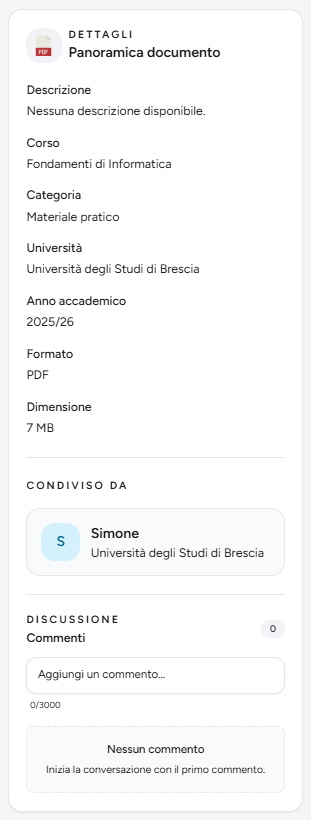
\includegraphics[width=0.3\textwidth]{figures/fig-riprogettazione-fisica/visualizzazione-documento/visualizzazione_documento_1.png}
    \caption{}
    \label{fig:visualizzazione-documento-1}
  \end{figure}

  \item \textbf{Infinite List} (Tidwell): Il pattern descrive la gestione di elenchi di dati tramite uno scorrimento che mantiene l'utente all'interno dello stesso contesto visivo, spesso preferito alla paginazione tradizionale per non interrompere il flusso dell'attività. È stato associato questo approccio alla \textit{Progressive Disclosure}, che consiste nel mostrare inizialmente solo le informazioni essenziali (come i primi commenti) e svelare il resto solo su richiesta dell'utente per evitare il "sovraccarico cognitivo".  

  Problemi di usabilità risolti:
  \begin{itemize}
    \item P79 (I commenti non sono paginati e rallentano la pagina): È stata implementata una visualizzazione progressiva (mostrando ad esempio "5 commenti di 6") con un tasto "Mostra altro". Al superamento dei 10 commenti, l'area diventa scorrevole internamente tramite uno scroll dedicato, evitando che la pagina si allunghi eccessivamente e diventi lenta nel caricamento.
  \end{itemize}

  \begin{figure}[H]
    \centering
    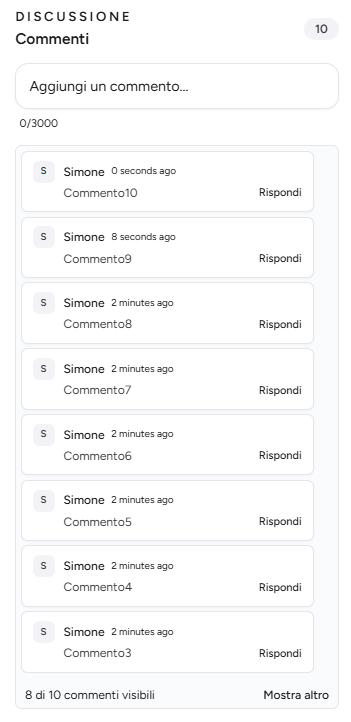
\includegraphics[width=0.3\textwidth]{figures/fig-riprogettazione-fisica/visualizzazione-documento/commenti.png}
    \caption{}
    \label{fig:commenti}
  \end{figure}

\end{itemize}

\paragraph{Altre modifiche}
Sono state apportate correzioni puntuali per migliorare la coerenza del sistema e la sicurezza della community. Sono stati rimossi i feedback visivi ingannevoli che suggerivano interattività dove non presente e sono stati uniformati i testi dei pulsanti per garantire che il linguaggio dell'interfaccia rifletta sempre l'azione che l'utente sta per compiere. È stato inoltre migliorato il sistema di gestione dei file scaricati e introdotto un controllo preventivo sui contenuti per garantire un ambiente di studio adeguato. \\  

Problemi di usabilità risolti:
\begin{itemize}
\item P34 (La voce ”Corso” non è cliccabile): La riga è stata trasformata in semplice testo informativo all'interno della descrizione del documento, eliminando il falso link che creava confusione.
\item P55 (Inconsistenza terminologica ”Scarica” vs ”download”): Il termine è stato uniformato in ”Scarica” sia nella visualizzazione a lista che nel dettaglio del documento, rispettando il principio di coerenza linguistica.
\item P62 (Impossibile segnalare un commento o documento inappropriato): È stata implementata una blacklist di parole non adeguate che impedisce l'invio di commenti offensivi alla radice, proteggendo la community; si tratta di una misura di primo livello, non esaustiva, che intercetta i casi più evidenti.
\item P64 (Il file scaricato ha un nome casuale): Ora il file viene salvato utilizzando il titolo inserito dall'utente durante il caricamento, rendendo il materiale facilmente riconoscibile sul dispositivo dopo il download.
\end{itemize}  

\begin{figure}[H]
  \centering
  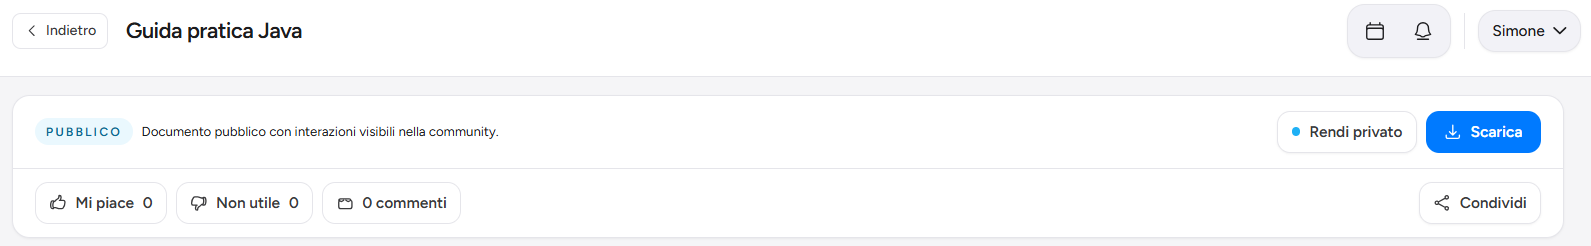
\includegraphics[width=0.8\textwidth]{figures/fig-riprogettazione-fisica/visualizzazione-documento/visualizzazione_documento_2.png}
  \caption{}
  \label{fig:visualizzazione-documento-2}
\end{figure}